\documentclass{article}

\usepackage{longtable}

\usepackage{indentfirst}

\usepackage[utf8]{inputenc}
\usepackage[T1]{fontenc}
\usepackage{fancyhdr}
\usepackage{geometry}
\usepackage{array}
\usepackage[usenames,dvipsnames,svgnames,table]{xcolor}
\usepackage{multirow}
\usepackage{morefloats}
\usepackage{float}
\usepackage{soul}
\usepackage{color}
\usepackage{seqsplit}
\usepackage{gensymb}
\usepackage{siunitx}
\usepackage{graphicx}
\usepackage{pdfpages}
\usepackage[framemethod=TikZ]{mdframed}
\setcounter{secnumdepth}{3}

\usepackage[procnames]{listings}
\usepackage{color}

\definecolor{keywords}{RGB}{255,0,90}
\definecolor{comments}{RGB}{0,0,113}
\definecolor{red}{RGB}{160,0,0}
\definecolor{green}{RGB}{0,150,0}

\lstset{language=Python,
        basicstyle=\ttfamily\small,
        keywordstyle=\color{keywords},
        commentstyle=\color{comments},
        stringstyle=\color{red},
        % showstringspaces=false,
        identifierstyle=\color{green},
        procnamekeys={def,class}}


\restylefloat{table}

\fontfamily{cmss}\selectfont

\geometry{top = 1in, bottom = 1in, left = 0.5in, right = 0.5in}

\setlength{\parindent}{4em}
\setlength{\parskip}{1em}
\renewcommand{\baselinestretch}{1.5}

\pagestyle{fancy}
\renewcommand{\footrulewidth}{1pt}
\lhead{Waggle Sensor Array}
\chead{Rain Gauge and Soil Moisture Sensor}
\rhead{Version 0.1 alpha 1}
\lfoot{Waggle Group}
\rfoot{info@wa8.gl, park708@purdue.edu}

\setlength{\tabcolsep}{10pt}
\renewcommand{\arraystretch}{1.0}

%%%%%%%%%%%%%%%%%%%%%%%%%%%%%%%%%%%%%%%%%%%%%%%%%%%%%%%%%%%%%%%%%%%%%%%%%%%%

\begin{document}

\begin{titlepage}
   \vspace*{\stretch{1.0}}
   \begin{center}
        \Huge\textbf{\textsc{Data Format Specification \\ for Rain Gauge \\ and Soil Moisture Sensor}} \\
        % \Large\textsc(v3 sensor boards)}}\\[0.5cm]
        \Large\textsc{Waggle Group \\ Waggle Sensor Array}\\[1cm]
        \large\textsc{January 2017, }
        \large\textsc{Version 0.1 alpha 1}\\
   \end{center}
   \vspace*{\stretch{2.5}}
\end{titlepage}

\tableofcontents
\newpage

\section{Physical Connections and Interfaces}

`v3 sensor boards and rain gauge' means a set of sensors which includs a v3.1 Metsense board, a v3.1 Lightsense board, a Chemsense board, and Rain Gauge.
In this section, we will only deal with physical connection between Rain Gauge and Metsense board.
\par

Physical connections between a Metsense board and a rain gauge are shown in the Figure \ref{fig:connect}. A rain gauge is connected to Metsense board directly through wires. The connection between the rain gauge and Metsense board is detected through an analog read signal through pin 2 of 3V3AD. When zero voltage, ground, is connected to Pin 2 of 3V3AD, sensor board notice that a rain gauge is connected. Therefore, the ground line from rain gauge need to be connected to both pin 1, which is ground, and 2 of 3V3AD simultaneously. The rain gauge deliver data through pin 2 of JP2, digital up/down signal.



\begin{figure}[h]
\begin{center}
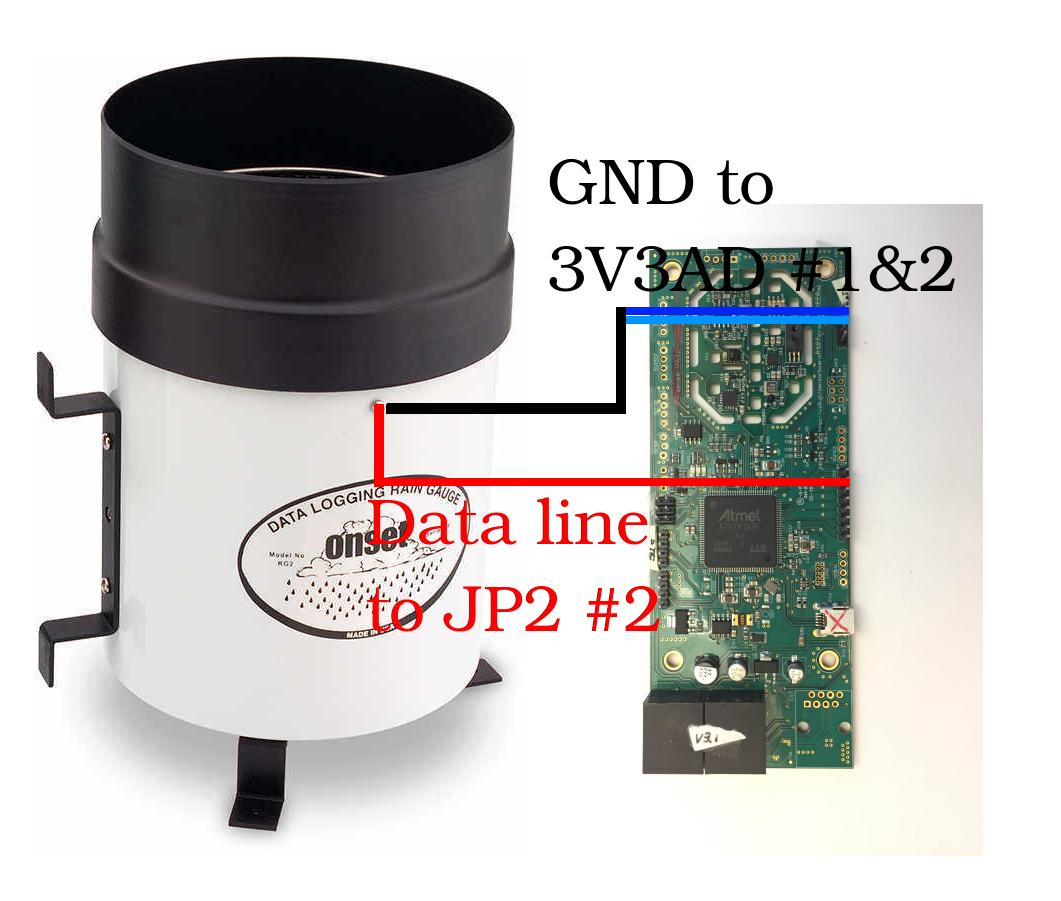
\includegraphics[width=4in]{con.png}
\caption{Connections between a Metsense board and a rain gauge}
\label{fig:connect}
\end{center}
\end{figure}

Detail wireing to the rain gauge and board is shown in Figure \ref{fig:gauge_in} - \ref{fig:gauge_board}. Wire from the rain gauge as shown in Figure \ref{fig:gauge_in} is going out though a hole of the body of the rain gauge as shown in Figure \ref{fig:gauge_out}, and connected to the board as shown in Figure \ref{fig:connect}. Before the two lines from the rain gauge are connected to the Metsense board, the ground line need to be distinguished. You can use a multimeter to find one. Set a multimeter to measure voltage, connect each of the line to probes of the multimeter and move a tick inside of the rain gauge. Then you can tell which one is ground.
\par
Pin detail of the Metsense board is shown in Figure \ref{fig:gauge_board}. Deep blue squre marked in Figure \ref{fig:gauge_board} is a ground pin, and light blue squre is a connection pin. The connection pin and gound line of rain gauge need to be connected to the ground pin. Data pin marked as a red squre need to be connected to data line of rain gauge.


\makeatletter
\setlength{\@fptop}{0pt}
\makeatother


\begin{figure}[!htb]
\minipage{0.32\textwidth}
  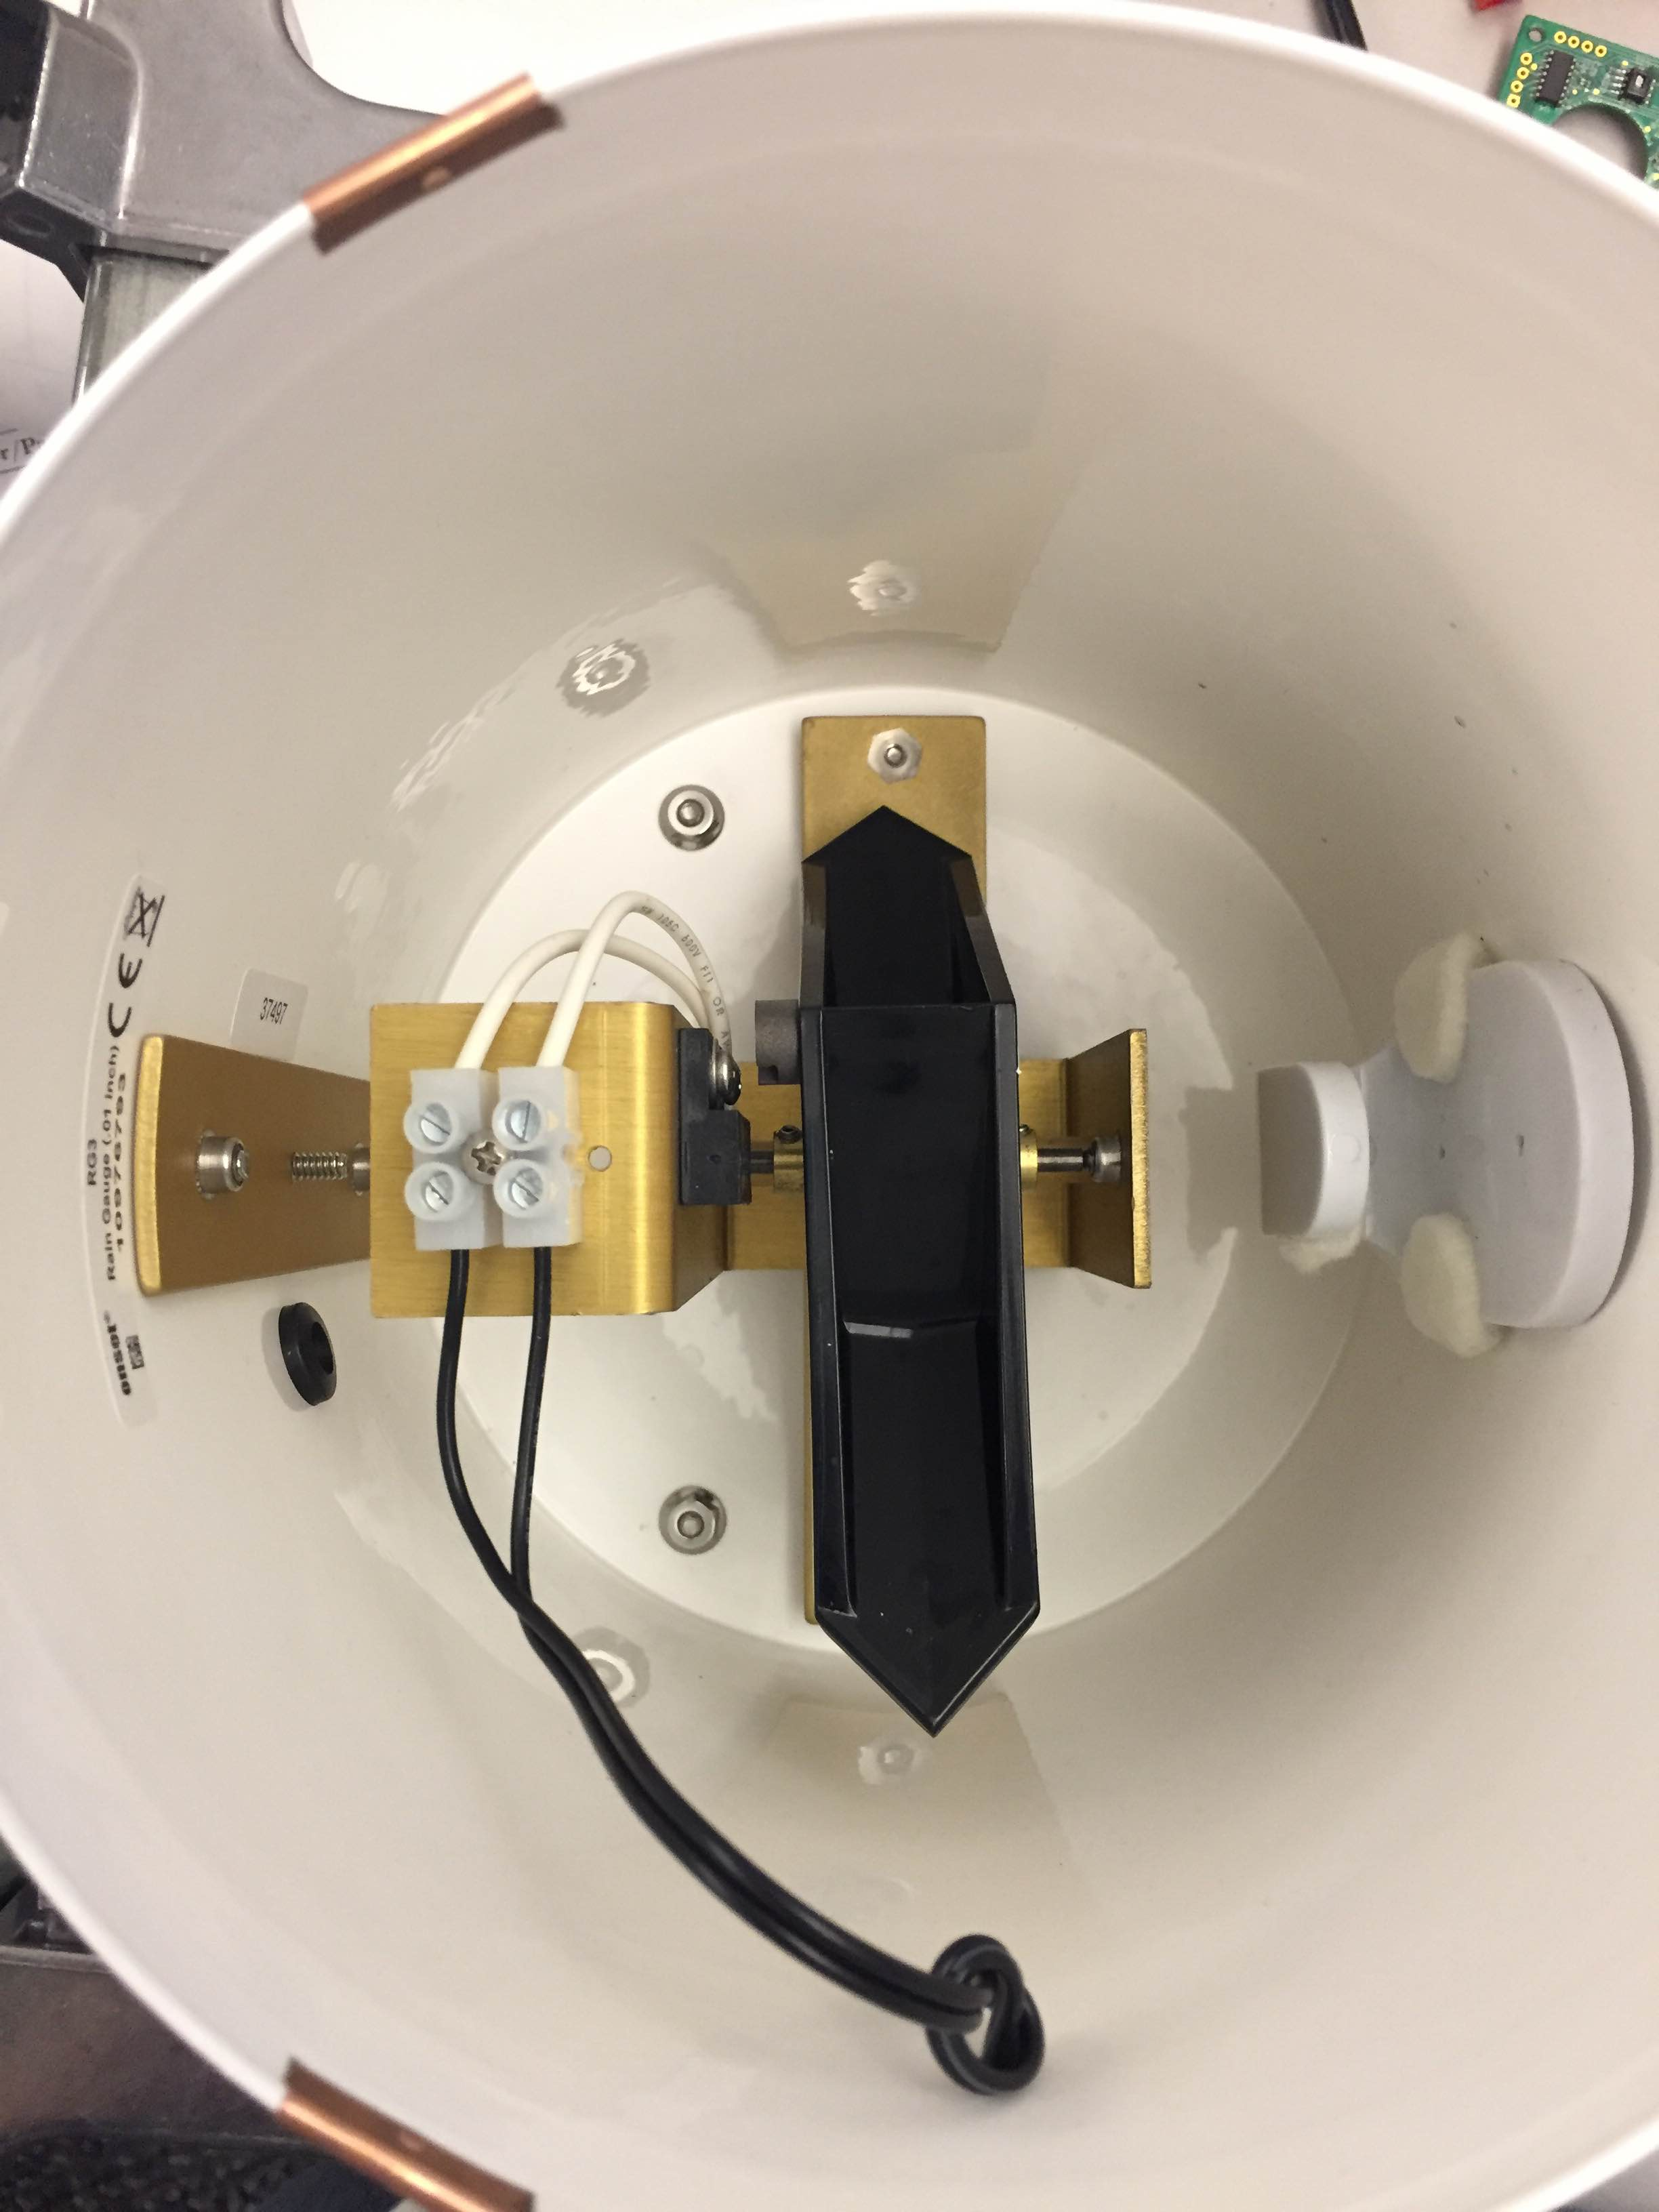
\includegraphics[width=\linewidth]{in.png}
  \caption{Connections inside of the rain gauge}
  \label{fig:gauge_in}
\endminipage\hfill
\minipage{0.32\textwidth}
  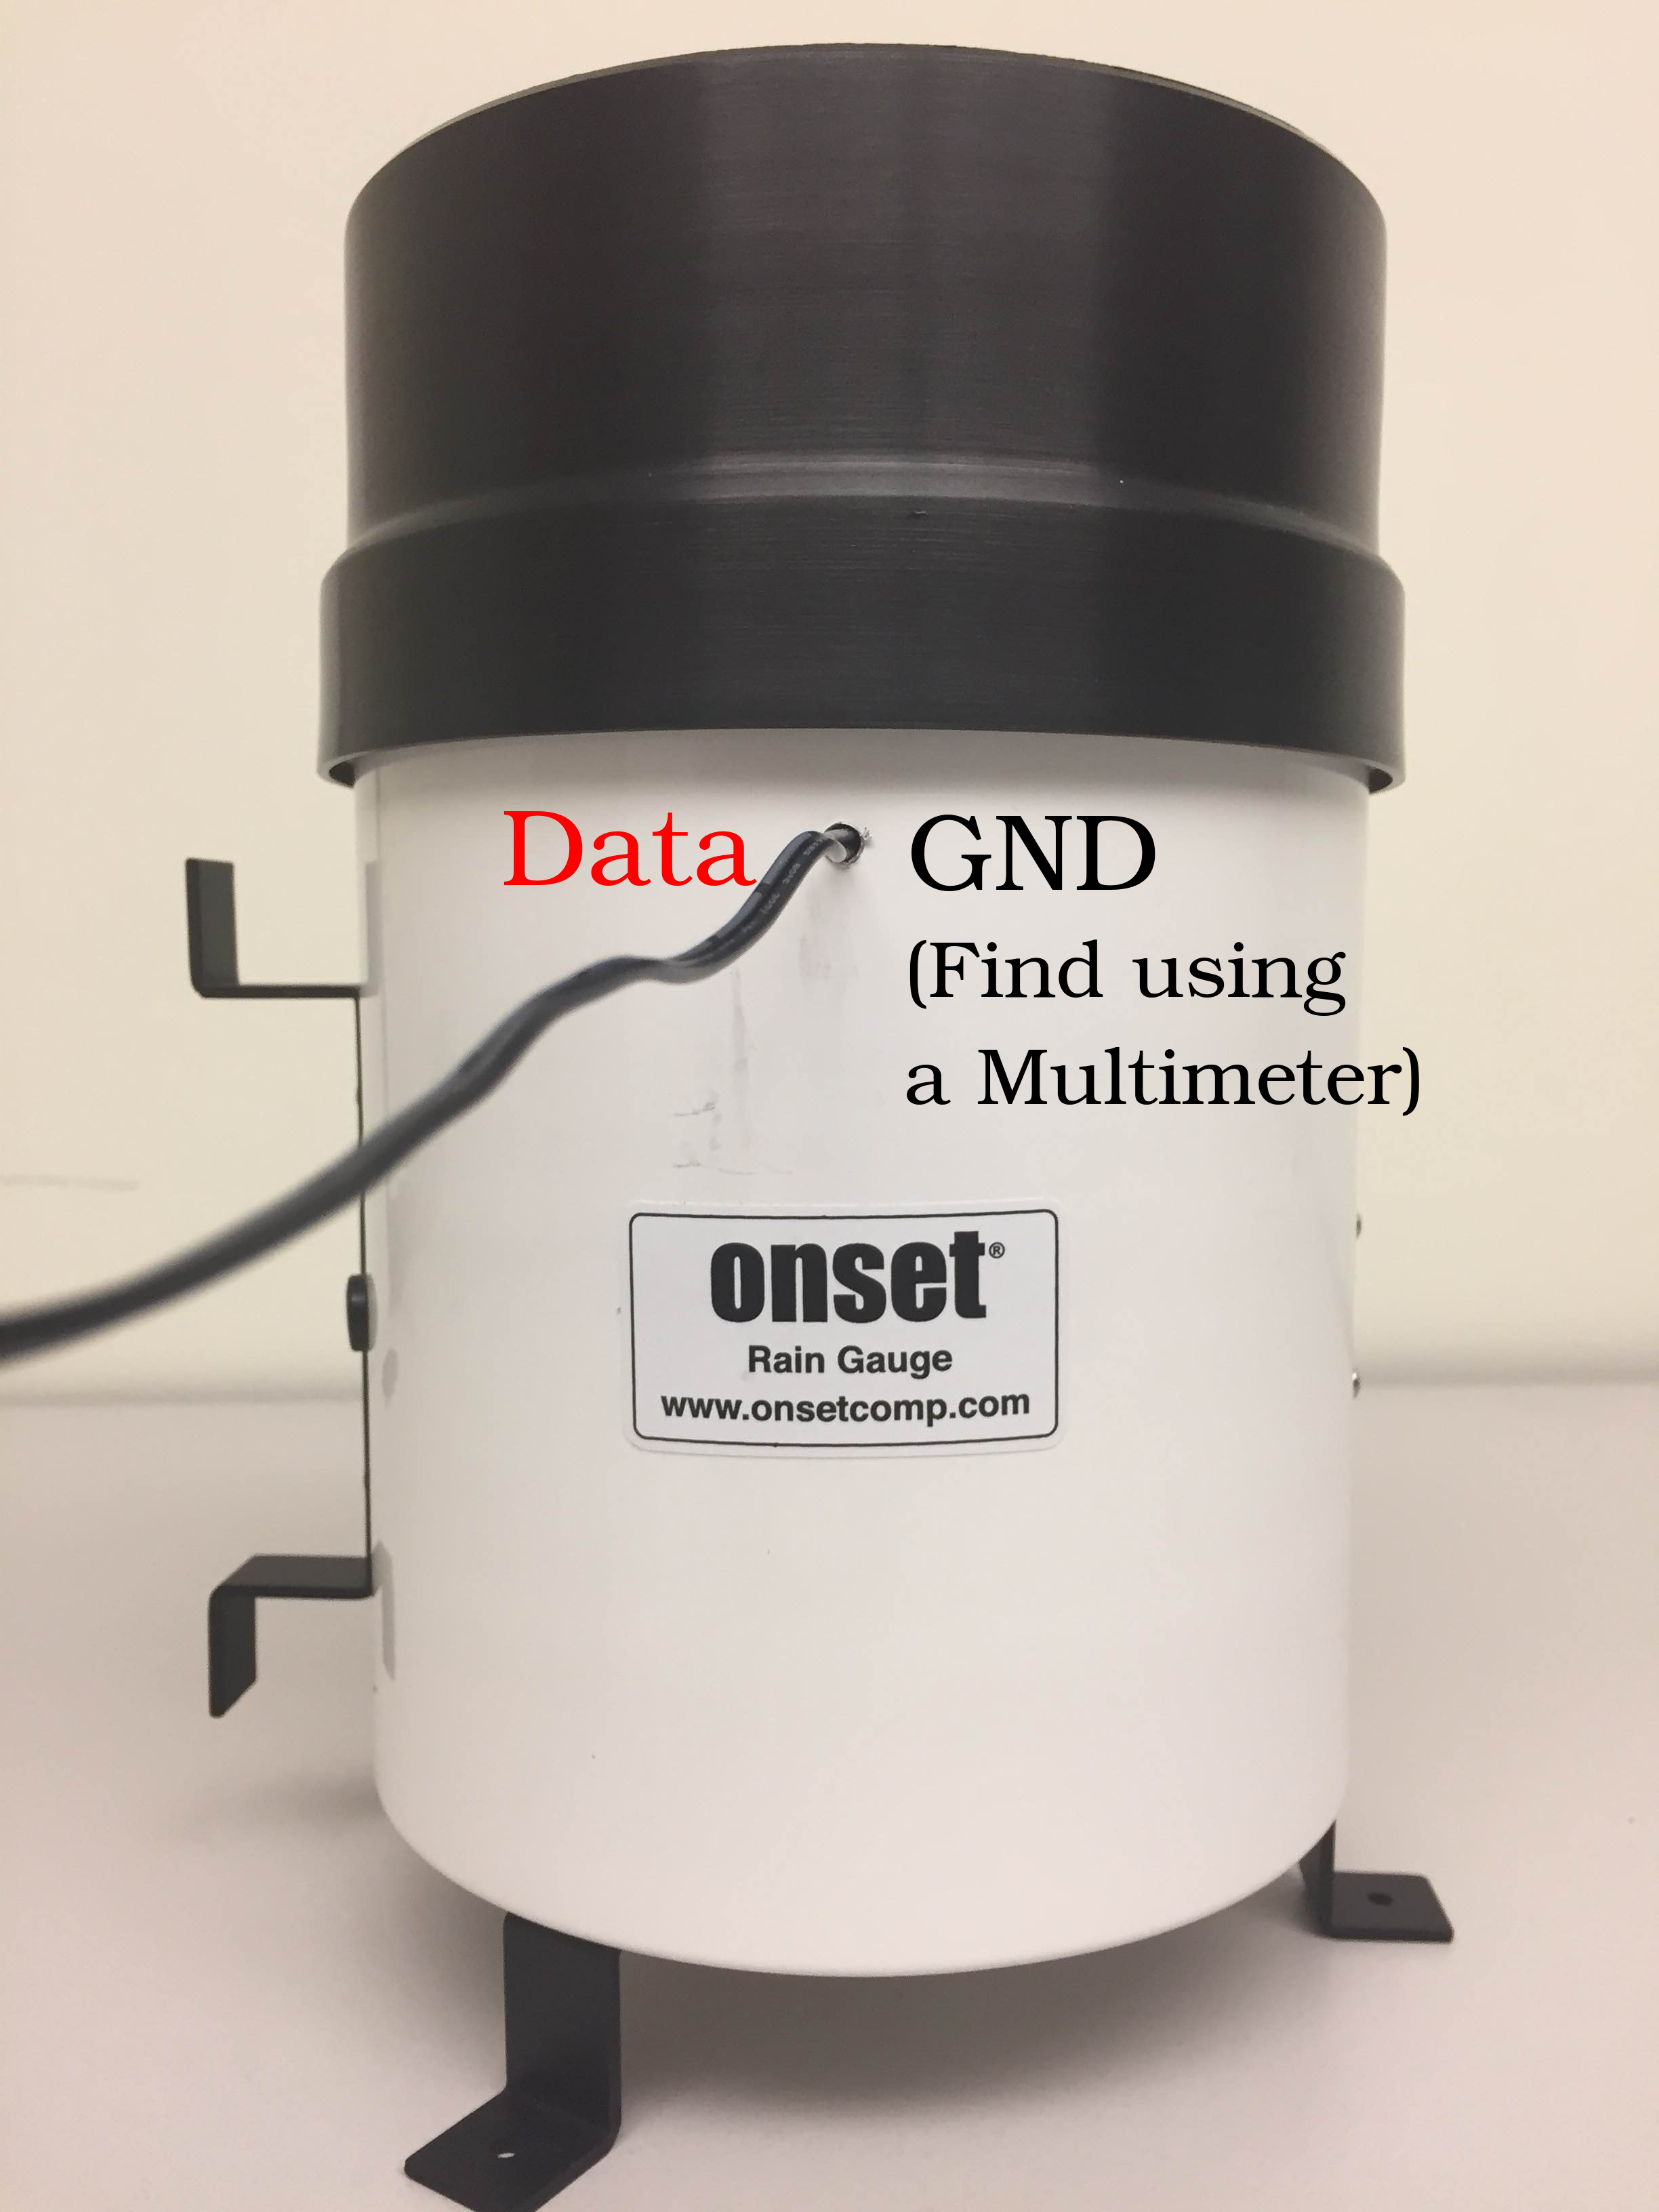
\includegraphics[width=\linewidth]{gauge.png}
  \caption{Connections outside of the rain gause}
  \label{fig:gauge_out}
\endminipage\hfill
\minipage{0.32\textwidth}%
  \includegraphics[width=\linewidth]{a.png}
  \caption{Connections to the Metsense board}
  \label{fig:gauge_board}
\endminipage
\end{figure}

\clearpage
\newpage
\section{Data Transmission} \label{section:overall}

The data from the sensor boards is sent as a formatted unit of data -- a transmission
packet. A transmission packet is composed of several data sub-packets, each
of which carries information pertaining to the parameter.
The transmission packet format and the data sub-packets are described here.

\subsection{Transmission Packet}
A transmission packet can be separated into 6 segments.
The structure of the transmission packet relies on positions of Bytes and predefined values for those Byte segments. 
Table 1 below illustrates how the segments are organized in a transmission packet.
\\

\begin{table}[h!]
    \centering
    \caption{Transmission Packet structure}
    \label{table:tran}
    \begin{tabular}{|c|c|c|c|c|c|}
        \hline
        \rowcolor{black!8}
        \textbf{Preamble} & \textbf{Seq. | Prot. Ver.} & \textbf{Data Length} & \textbf{Data} & \textbf{CRC} & \textbf{Postscript}\\
        \hline
        \multirow{2}{*}{1st Byte} & \multirow{2}{*}{2nd Byte} & \multirow{2}{*}{3rd Byte} & next Bytes & \multirow{2}{*}{Penultimate Byte} & \multirow{2}{*}{Final Byte} \\ 
        & & & up to 251 Bytes & & \\ \hline
    \end{tabular}
\end{table}


The first segment is the start byte, or the preamble. The preamble is followed by the packet sequence number and protocol
version, each of which are 4 bits long and are together packed into a single byte.
Next, one byte field that reports the length of the data which follows it
immediately. The data segment is followed by a single CRC byte, and finally the packet ends with a one byte
postscript. Table \ref{table:seg} lists the packet and the static values, if any, for each of the segments.
\\


\begin{table}[H]
    \centering
    {
    \begin{tabular}{|c|c|c|c|}
        \hline
        \rowcolor{black!8}
        \textbf{Field} & \textbf{Value} & \textbf{Segment} & \textbf{Length}\\
        \hline
        Preamble & 0xAA & 1 & 1 Byte\\ \hline
        Packet Sequence Number & Variable & \multirow{2}{*}{2} & 1 Nibble\\ \cline{1-2} \cline{4-4}
        Protocol version & 0x00 &  & 1 Nibble\\ \hline
        Length of data (not whole packet) & Variable & 3 & 1 Byte\\ \hline
        Data & Variable & 4 & Variable \\ \hline
        CRC of data (not whole packet) & Variable & 5 & 1 Byte\\ \hline
        Postscript & 0x55 & 6 & 1 Byte\\ \hline
    \end{tabular}
    }
    \caption{Transmission Packet Segments}
    \label{table:seg}
\end{table}


\subsection{Data Sub-packets} \label{ssec:sub-pack}

The data segment of the transmission packet is further separated into many
sub-packets. Table \ref{table:packsegments} below shows the organization
of a sub-packet.
The sub-packet starts with a source identifier. One bit
validity field and seven bits ``length of the sub-packet'' field
are packed together as the next byte. The length field counts the number of
bytes following it which make up the sub-packet, and also counts Bytes of a source identifier and the length field. 
The validity bit is set to 1 if the sensor reading is valid and set to 0 if the sensor
is dead, disabled, unconnected, unresponsive or if data could not be collected
from the sensor in the time window. The size of the sub-packet is restricted to 127 Bytes by the seven bits length field.
\par
The packet validity is initially 0, and it will be changed to 1 when each sub-packet gets sensor value from sensor. 
And after a transmission packet is trasmitted, the validity becomes 0 again. 
When validity is set to 0, if the sensor is dead, disabled, unconnected, unresponsive or data could not be collected,
the particular invalid sub-packet is not packed into a transmission packet.
\\

\begin{table}[H]
    \centering
    {
    \begin{tabular}{|c|c|c|}
        \hline
        \rowcolor{black!8}
        \textbf{Source ID} & \bf{1-bit Validity [0: invalid, 1: valid]| 7-bits Data Length} & \textbf{Data} \\ \hline
        1 Byte & 1 Byte & up to 127 Bytes \\
        \hline
    \end{tabular}
    }
    \caption{Transmission Packet Segments}
    \label{table:packsegments}
\end{table}




\subsection{Data Packer CRC} \label{ssec:crc-calc}

To validate the data transmitted from the sensor board, a CRC value for the data is
calculated and transmitted as part of the data packet. The Maxim 1-Wire
CRC polynomial is used for calculating the CRC.  On receiving the data packet, the CRC
of the data packet is recalculated and compared with the value transmitted as part of
the packet. If the two CRC values match, the transmission is error-free.
The equivalent polynomial function of the CRC is shown in Equation \ref{eq:CRC}.

\begin{equation}
\label{eq:CRC}
CRC = x^8 + x^5 + x^4 + 1
\end{equation}

Further description of the Maxim 1-Wire CRC is available in Maxim Application Note 27. Below are
the Python and C implementations of the CRC calculator. The CRC implementations below take a
data Byte and the previous CRC as inputs, and return the new CRC as return value.
\\

\textbf{Python Code:}
\begin{mdframed}
\begin{lstlisting}
def calc_crc (data_Byte,CRC_Value)
    CRC_Value = ord(data_Byte) ^ CRC_Value
    for j in range(8):
    if (CRC_Value  & 0x01):
        CRC_Value  = (CRC_Value  >> 0x01) ^ 0x8C
    else:
        CRC_Value  =  CRC_Value  >> 0x01
return CRC_Value
\end{lstlisting}
\end{mdframed}

\vskip 0.1in
\textbf{C Code:}
\begin{mdframed}
\begin{lstlisting}
unsigned char  CRC_CALC (unsigned char data, unsigned char crc) 
{ 
        unsigned char i;
        crc ^= data;
        for (i=0x00; i < 0x08; i++)
        {
                if (crc & 0x01) { crc = (crc >> 0x01)^0x8C; }
                else { crc =  crc >> 0x01; }
        }
        return(crc);
}
\end{lstlisting}
\end{mdframed}
\newpage
\section{Sensor Data Units}\label{section:parameterUnits}
\subsection { Raw and Processed} 

\begin{center}
\rowcolors{2}{white}{black!5}
\begin{longtable}{|l|l|l|l|}
\caption{Sensor units both in raw and processed format}
\label{table:parameterUnits} \\

\hline \rowcolor{white} \multicolumn{1}{|l|}{\textbf{Sensor/Parameter}} & \multicolumn{1}{l|}{\textbf{Raw Units}} & \multicolumn{1}{l|}{\textbf{Processed Units}} & \multicolumn{1}{l|}{\textbf{Comments}} \\ \hline
\endfirsthead

\multicolumn{4}{c}%
{{\bfseries \tablename\ \thetable{} -- continued from previous page}} \\

\hline \rowcolor{white} \multicolumn{1}{|l|}{\textbf{Sensor/Parameter}} & \multicolumn{1}{l|}{\textbf{Raw Units}} & \multicolumn{1}{l|}{\textbf{Processed Units}} & \multicolumn{1}{l|}{\textbf{Comments}} \\ \hline
\endhead

\hline \rowcolor{white} \multicolumn{4}{|r|}{{Continued on next page}} \\ \hline
\endfoot

\hline \hline
\endlastfoot

% 
% \begin{table}[H]
%     \centering
%     {\rowcolors{2}{black!8}{black!2}
%     \begin{tabular}{|l l l l|}
%         \hline
%         \textbf{Sensor/Parameter} & \textbf{Raw Units} & \textbf{Processed Units} & \textbf{Comments}\\
%         \hline
%         \hline
    \hline \rowcolor{white} \multicolumn{4}{|c|}{{Airsense board}} \\ \hline
    Air/Lightsense MAC & No Units & No Units & \\ % 6 Octets in hex notation separated by `:'\\
    TMP112 & \degree C & \degree C & \\
    HTU21D & \degree C, \%RH & \degree C, \%RH & \\
    HIH4030 & \%RH & \%RH & \\
    BMP180 & \degree C, Pa & \degree C, Pa & \\
    PR103J2 & integer & \degree C & \\
    TSL250RD & integer & $\mu$w/m$^2$ & \\ % **finalize after discussion with EVS** \\
    MMA8452Q & g, g, g, g & g, g, g, g & \\
    SPV1840LR5H-B & & & which pin does the sensor is using?\\ % integer & dB & \\
    TSYS01 & \degree C & \degree C & \\
    
    \hline \rowcolor{white} \multicolumn{4}{|c|}{{Lightsense board}} \\ \hline
    HMC5883L & G, G, G & G, G, G & \\
    HIH6130 & \degree C, \%RH & \degree C, \%RH & \\
    APDS-9006-020 & integer & lux & \\ % **finalize after discussion with EVS**\\
    TSL260RD & integer & $\mu$w/m$^2$ & \\ % **finalize after discussion with EVS** \\
    TSL250RD & integer & $\mu$w/m$^2$ & \\ % **finalize after discussion with EVS** \\
    MLX75305 & integer & $\mu$w/m$^2$ & \\ % **finalize after discussion with EVS** \\
    ML8511 & integer & $\mu$w/m$^2$ & \\ % **finalize after discussion with EVS** \\
%     D6T & \textit{Seventeen} \degree C values & \textit{Seventeen} \degree C values & \\
%    MLX90614 & \degree F & \degree C & \\
    TMP421 & \degree C & \degree C & \\
%     SPV1840LR5H-B & integer & dB & \\

    \hline \rowcolor{white} \multicolumn{4}{|c|}{{Chemsense board}} \\ \hline
    Total reducing gases & AFE ADC counts & & data not yet processed \\ % integer & concentration & **finalize after discussion with EVS**\\
%     Ethanol & integer & ppm & Quadratic equation with calibrated weights \\
    Nitrogen dioxide & AFE ADC counts & & data not yet processed \\ % integer & ppm & Quadratic equation with calibrated weights\\
    Ozone & AFE ADC counts & & data not yet processed \\ % integer & ppm & Quadratic equation with calibrated weights\\
    Hydrogen sulphide & AFE ADC counts & & data not yet processed \\ % integer & ppm & Quadratic equation with calibrated weights\\
    Total oxidizing gases & AFE ADC counts & & data not yet processed \\ % integer & concentration & **finalize after discussion with EVS**\\
    Carbon monoxide & AFE ADC counts & & data not yet processed \\ % integer & ppm & Quadratic equation with calibrated weights\\
    Sulfur dioxide & AFE ADC counts & & data not yet processed \\ % integer & ppm & Quadratic equation with calibrated weights\\
    Sensirion (SHT25) & 100ths of \degree C, 100ths of \%RH & \degree C, \%RH & \\ % \degree C, RH \% & \degree C, RH \% & \\
    LPS25H & 100ths of \degree C, Pa & \degree C, Pa & \\ % \degree C $\times$ 100, RH \% & \degree C, RH \% & \\
    Si1145 & fixed value & & firmware is not completed \\
%     Bosh & hPa& hPa & \\
    Intel MAC address & No Units & No Units & \\ % 6 Octets in hex notation separated by `:'\\
%     Sensor status (health) & No Units & No Units & 4 bytes of sensor health data\\
    CO ADV temp & 100ths of \degree C & \degree C & \\
    IAQ IRR ADC temp & 100ths of \degree C & \degree C & \\
    O3 NO2 ADC temp & 100ths of \degree C & \degree C & \\
    SO2 H2S ADC temp & 100ths of \degree C & \degree C & \\
    CO LMP temp & 100ths of \degree C & \degree C & \\
    Accelerometer & Raw register & & data not yet processed \\
    Gyro & Raw register & & data not yet processed \\
    
    \hline \rowcolor{white} \multicolumn{4}{|c|}{{Alpha sensor}} \\ \hline
    Histogram & & & \\
    Firmware & & & \\
    Configuration & & & \\
    \hline
%     \end{tabular}
%     }
%     \caption{Sensor and Parameter units both in raw and processed format.}
%     \label{table:parameterUnits}
% \end{table}
\end{longtable}
\end{center}


\subsection{ conversion processure}

\subsection{Airsense:}
\subsubsection{ TMP112} \label{ssec:first}

Raw ouput of TMP112 is a digital 12-bit value. Coresensor firmware calculates temperature in centigrade using 12-bits of two Bytes reading of the sensor output. \\

{\centering
  temperature \((\degree C)\) = usigned integer form of 12-bit digital output $\times$ 0.0625\par
}

\bigbreak
The equation refers the resolution for the Temperature ADC in Internal Temperature mode which is 0.0625 \(\degree C/count\).

\subsubsection{ HTU21D}
Raw output values of HTU21D are digital 12-bits / 8-bits (for Temperature / relative humidity) from default configuration. Coresensor firmware calculates  temperature and humidity in centigrade and relative humidity using relevant bits of two Bytes reading of the sensor output.

{\centering
 \[ \text{temperature \((\degree C)\)} = \frac{\text{usigned integer form of digital output}}{2^{16}} \times 175.72 - 46.85 \] 
 \[ \text{humidity \((\%RH)\)} = \frac{\text{usigned integer form of digital output}}{2^{16}} \times 125 - 6 \]
 \par
 }

\bigbreak
 The calculated humidity is re-calculated in sensor plugin using temperature coefficient compensation equation. \\

{\centering
 humidity \((\%RH)\) = unsigned integer form of  - (25 - temperature) $\times$ 0.15
 \par
}

\bigbreak
The equation refers temperature coefficient of the HTU21D(F) in 0.15 \(\%RH/\degree C\).

\subsubsection{ HIH4030}

Raw output of HIH4030 is an interger indicating output voltage from the sensor which is mapped into an integer value between 0 and 1023. Output voltages between 0 and 5 volts from the sensor will be mapped into integer values between 0 and 1023. Coresensor firmware delivers the two Bytes of raw integer value, and coresense plugin calculates humidity using output voltage from the sensor.

{\centering
 \[ \text{output voltage \((V)\)} = \frac{\text{usinged integer raw output} \times 5}{1023} \] 
 \[ \text{humidity \((\%RH)\)} = (\text{output voltage} - 0.85) \times \frac{100}{3} \]
 \par
 }
\bigbreak
The slope term (\(\frac{100}{3}\)) and y-intercept (0.85) are comming from a graph given in the HIH4030 sensor datasheet (figure 4). This slope and y-intercept can be different depending on temperature.

\subsubsection{ BMP180}

Raw ouput values of BMP180 are 16-bit/24-bit value (temperature/pressure), and the values are post-processed through a library provided by Adafruit Industries. Sensor output values from the coresensor firmware are temperature in centigrade and barometric pressure in pascal.


\subsubsection{ PR103J2}

Raw output of PR103J2 is an interger indicating output voltage from the sensor which is mapped into integer values between 0 and 1023. Output voltages between 0 and 5 volts from the sensor will be mapped into integer values between 0 and 1023. Coresensor firmware delivers the two Bytes of raw integer value, and coresensor plugin calculates temperature using output voltage from the sensor and resistance-temperature look-up table (PR103J2 R-T table).

{\centering
 \[ \text{output voltage } (V) = \frac{\text{usinged integer raw output} \times 5}{1023} \] 
 \[ \text{resistance } (\Omega) = 47000 \times \left(\frac{1023}{\text{voltage}} - 1\right) \]
 \par
 }


\subsubsection{ TSL250RD}

What we can get from TSL250RD in airsense board as a raw output is an interger indicating output voltage from the sensor which is mapped into integer values between 0 and 1023. Output voltages between 0 and 5 volts from the sensor will be mapped into integer values between 0 and 1023. Coresensor firmware delivers the two Bytes of raw integer value, and coresensor plugin calculates irradiance of visible light in micro-watt per square meter.

{\centering
 \[ \text{output voltage }(V) = \frac{\text{usinged integer raw output} \times 5}{1023} \] 
 \[ \text{irradiance } (\mu W/m^2) = \frac{\text{output voltage} - 0.09}{0.064} \]
 \par
 }
 
\bigbreak
The equation refers irradiance responsivity of TSL250RD which is 0.064 \(mV/(\mu W/cm^2\)), and 0.09 is output voltage of dark condition which is initial offset (without any light -- NEED TO BE CHECKED).

\subsubsection{ MMA8452Q}

Raw ouput values of MMA8452Q are actual g value, this depends on scale being set.

\subsubsection{ SPV1840LR5H-B}

\subsubsection{ TSYS01}

Raw ouput value of TSYS01 is post-processed value through a library provided by  Free Software Foundation, Inc.. Sensor output from the coresensor firmware is temperature in centigrade.


\subsection{Lightsense:}
\subsubsection{ HMC5883L}

Raw ouput values of HMC5883L are post-processed values through a library provided by Adafruit Industries. Sensor output values from the coresensor firmware are acceleration values in Gauss.

\subsubsection{ HIH6130}

Raw ouput values of HIH6130 are 14-bit temperature and humidity values. Coresensor firmware calculates temperature and humidity in centigrade and relative humidity using 14-bits of two Bytes reading of the sensor output.

{\centering
 \[ \text{temperature (\degree C)} = \frac{\text{usigned integer form of digital output}}{2^{14} - 2} \times 165 - 40 \] 
 \[ \text{humidity (\%RH)} = \frac{\text{usigned integer form of digital output}}{2^{14} - 2} \times 100 \]
 \par
 }


\subsubsection[MCP3426]{ APDS-9006-020, TSL260RD, TSL250RD, MLX75305, ML8511 : \\ using MCP3426}

Raw output value of MCP3426 is an digital output which is proportional to the input voltage and programmable gain amplifier (PGA) settings (see schematics v3.1). Default setting of PGA is x1, and we are using 16-bits resolution. Coresensor firmware delivers the two Bytes of raw integer value, and coresensor plugin calculates irradiance of light in micro-watt per square meter using voltage output from each sensor. The voltage value need to be calculated regarding to the airsense circuit schematics and output modification equation for MCP3426 circuit. Coresensor firmware delivers the two Bytes of raw integer value, and coresensor plugin calculates irradiance of visible light in a designated unit.

{\centering
 \[ \text{output voltage of MCP3426 }(V) = \frac{\text{unsigned integer form of digital output}}{\text{maximum 16-bit code} + 1} * \text{reference voltage} \]
 \[ \text{input voltage od MCP3426} = \frac{\text{output voltage of MCP3426} * 5}{2} \]
 \par
 }

\bigbreak
The equation refers maximum n-bit code which is \( 2^{n - 1} - 1 \), and in case of 16-bit code, the number is 32767. Also reference voltage of MCP3426 is 2.048 \(V\). According to schematics v3.1, the output voltage from each sensor is divided, so the original output voltage can be calculated by the equation given above.

\paragraph{a. APDS-9006-020}

Raw output value of APDS-9006-020 is an analog current which is proportional to the irradiance. The output current can be converted into voltage value according to the board schematics v3.1.

{\centering
 \[ \text{output current }(\mu A) = \frac{\text{input voltage to MCP3426}}{0.005} \] 
 \[ \text{irradiance } (lux) = {\text{output current} - 0.000156} * 2.5 \]
 \par
 }
 
\bigbreak
The equation refers resistance of 5 \(K \Omega \) which is used as 0.005 to calculate current with unit \(\mu A\) as shown in schematics v3.1. Also initial offset of the sensor is applied as 0.000156, and linear relationship factor as 2.5, however these sensor property can be changed base on experiments.
 
\paragraph{b. TSL260RD}

Raw output value of TSL260RD is an analog voltage which is inverse proportional to the irradiance. The output voltage from the sensor has been calculated though the equations given in section 5.4.3.

{\centering
 \[ \text{irradiance } (\mu W/m^2) = \frac{\text{output current} - 0.005313}{0.058} \]
 \par
 }
 
 \bigbreak
 The equation refers irradiance responsivity of TSL260RD which is 0.058 \(mV/(\mu W/cm^2\)), and 0.005313 is output voltage of dark condition, which is initial offset (without any light -- NEED TO BE CHECKED).
 

\paragraph{c. TSL250RD}

Raw output value of TSL250RD is an analog voltage which is inverse proportional to the irradiance. The output voltage from the sensor has been calculated though the equations given in section 5.4.3.

{\centering
 \[ \text{irradiance } (\mu W/m^2) = \frac{\text{output current} - 0.005313}{0.064} \]
 \par
 }
 
 \bigbreak
 The equation refers irradiance responsivity of TSL250RD which is 0.064 \(mV/(\mu W/cm^2\)), and 0.005313 is output voltage of dark condition, which is initial offset (without any light -- NEED TO BE CHECKED).

\paragraph{d. MLX75305}

Raw output value of MLX75305 is an analog voltage which is inverse proportional to the irradiance. The output voltage from the sensor has been calculated though the equations given in section 5.4.3.

{\centering
 \[ \text{irradiance } (\mu W/m^2) = \frac{\text{output current} - 0.0996}{0.007} \]
 \par
 }
 
 \bigbreak
 The equation refers irradiance responsivity of MLX75305 which is 0.007 \(mV/(\mu W/cm^2\)), and 0.0996 is output voltage of dark condition, which is initial offset (without any light -- NEED TO BE CHECKED).

\paragraph{e. ML8511}

Raw output value of ML8511 is an analog voltage which is proportional to the irradiance. The output voltage from the sensor has been calculated though the equations given in section 5.4.3.

{\centering
 \[ \text{irradiance } (\mu W/m^2) = (\text{output current} - 1.489) * 12.49 \]
 \par
 }
 
 \bigbreak
 The equation refers proportional factor which is 12.49 \(mV/(\mu W/cm^2\)), and 0.0996 is output voltage of dark condition, which is initial offset (without any light -- NEED TO BE CHECKED).

%\subsubsection{ MLX90614}

\subsubsection{ TMP421}

Raw ouput value of TMP421 is 16-bit value, and the value is post-processed through a library provided by Free Software Foundation, Inc.. Sensor output from the coresensor firmware is temperature in centigrade.

% \subsubsection{ Lightsense MAC address}

\subsection{Chemsense:}
\subsubsection{ Chmical sensors}

\begin{itemize}
  \item Total reducing gases
  \item Nitrogen dioxide
  \item Ozone
  \item Hydrogen sulphide
  \item Total oxidizing gases
  \item Carbon monoxide
  \item Sulfur dioxide
\end{itemize}


\subsubsection{ SHT25}

Raw output values of SHT25 through chemsense firmware are 100ths of temperature in centigrade and 100ths of humidity value.

{\centering
 \[ \text{temperature }(\degree C) = \frac{\text{output value}}{100} \]
 \[ \text{humidity }(\% RH) = \frac{\text{output value}}{100} \]
 \par
 }

\subsubsection{ LPS25H}

Raw output values of LPS25H through chemsense firmware are 100ths of temperature in centigrade and pressure in Pa.

{\centering 
 \[ \text{temperature }(\degree C) = \frac{\text{output value}}{100} \]
}

\subsubsection{ Si1145}

Si1145 is a light sensor, and Chemsense board firmware is not completed, so the fixed hex values need to be ignored (July 2016).

%%%%%%%%%%%%%%%%%%%%%%%%%%%%%%%%%%%%%%%%%%%%%%%%%%%%%%%%%%%%%%%%%%%%%%%%%%%%%%%%%%%%%%%%
\subsubsection{ ADC Temperatures}
Chemsense board measures temperature of sensor ADCs. All of them give ADC temperature in 100ths of degree celsious. This includes five parameters which are:
 
\begin{itemize}
  \item CO ADC Temp
  \item IAQ/IRR ADC Temp
  \item O3/NO2 ADC Temp
  \item SO2/H2S ADC Temp
  \item CO CMT Temp
\end{itemize}


{\centering 
 \[ \text{temperature }(\degree C) = \frac{\text{output value}}{100} \]
}

\subsubsection{ Accelerometer}

\subsubsection{ Gyro}

\subsection{Alpha Sensor:}
\subsubsection{ Histogram}

\subsubsection{ Firmware}

\subsubsection{ Configuration}
\end{document}
